%!TEX root = IntroArithGrps.tex

\mychapter{Quasi-Isometries}
\label{QuasiChap}

\prereqs{none.}


\section{Word metric and quasi-isometries} \label{WordMetricSect}

The field of \term{Geometric Group Theory} equips groups with a metric, which allows them to be studied as metric spaces:

\begin{defn} \label{WordMetricDefn}
Fix a finite generating set~$S$ of~$\Gamma$ \csee{GammaFinGen}, and assume, for simplicity, that $S$ is \defit[symmetric!generating set]{symmetric}, which means $s^{-1} \in S$ for every $s \in S$.
\noprelistbreak 
	\begin{enumerate}
	\item For $g \in \Gamma$, the \defit[word!length]{word length} of~$g$ is the length~$\ell$ of the shortest sequence $(s_1,s_2,\ldots,s_\ell)$ of elements of~$S$, such that $s_1s_2\cdots s_\ell = g$. It is denoted $\ell(g)$.
	(By convention, $\ell(e) = 0$.)
	\item For $g,h \in \Gamma$, we let $d(g,h) = \ell(g^{-1} h)$. This defines a metric on~$\Gamma$, called the \defit[word!metric]{word metric} \csee{WordMetricEx}.
	%So $\Gamma$ is a metric space.
	\end{enumerate}
\end{defn}

The word metric has the important property that the action of~$\Gamma$ on itself by left-translations is an action by isometries \csee{LeftTransIsom}.

\begin{rem}
The word metric can be pictured geometrically, by constructing a \defit[Cayley!graph]{Cayley graph}. Namely, $\Cay(\Gamma; S)$ is a certain $1$-dimensional simplicial complex (or ``graph''):
	\begin{itemize} 
	\item its $0$-skeleton is~$\Gamma$,
	and
	\item it has a $1$-simplex (or ``edge'') of length~$1$ joining $v$ to~$vs$, for every $v \in \Gamma$ and $s \in S$.
	\end{itemize}
Define a metric on $\Cay(\Gamma; S)$ by letting $d(x,y)$ be the length of the shortest path from~$x$ to~$y$. Then the restriction of this metric to the $0$-skeleton is precisely the word metric on~$\Gamma$.
\end{rem}

Unfortunately, the word metric on~$\Gamma$ is not canonical, because it depends on the choice of the generating set~$S$ \csee{WordMetricNotWellDefd}. However, it is ``almost'' well-defined, in that changing the generating set can only distort the distances by a bounded factor. This idea is formalized in the following notion:

\begin{defn} \label{QuasiIsomDefn}
 Let $X_1$ and~$X_2$ be metric spaces, with metrics~$d_1$ and~$d_2$, respectively. 
 	\begin{enumerate}
	\item A function $f \colon X_1 \to X_2$ is a \defit[quasi-!isometry]{quasi-isometry} if there is a constant $C > 0$, such that
		 \begin{enumerate}
		 \item
		 for all $x,y \in X_1$ with $d_1(x,y) > C$,
		we have
		 $$ \frac{1}{C}
		 < \frac{ d_2 \bigl( f(x), f(y) \bigr) }
		 { d_1 ( x, y) }
		 < C ,$$ and
		 \item for all $x_2 \in X_2$, there exists $x_1 \in
		X_1$, such that 
			$$d_2 \bigl( f(x_1), x_2 \bigr) < C .$$
		 \end{enumerate}
 	Note that $f$ need not be continuous (and need not be one-to-one or onto, either).
	
	\item We say $X_1$ is \defit[quasi-!isometric]{quasi-isometric} to~$X_2$ (and write $X_1 \QI X_2$) if there is a quasi-isometry from~$X_1$ to~$X_2$. This is an equivalence relation \csee{QIEquivRel}.
	\end{enumerate}
 \end{defn}

\begin{prop}[\csee{WordWellDefEx}] \label{WordWellDef}
Let 
	\begin{itemize}
	\item $S_1$ and~$S_2$ be two finite, symmetric generating sets for~$\Gamma$,
	and
	\item $d_i$ be the word metric on~$\Gamma$ corresponding to the generating set~$S_i$.
	\end{itemize}
Then $(\Gamma,d_1) \QI (\Gamma,d_2)$.
\end{prop}

Therefore, if $\Gamma_1$ and~$\Gamma_2$ are quasi-isometric for some choice of the word metrics on the two groups, then they are quasi-isometric for all choices of the word metrics. So it makes sense to say that two groups are quasi-isometric, without any mention of generating sets (as long as both of the groups are finitely generated).

\begin{rem}
A property is said to be \defit[geometric property]{geometric} if is is invariant under quasi-isometry. For example, we will see (in \cref{AmenQIinvt,TnotQI}, respectively) that amenability is a geometric property, but Kazhdan's property~$(T)$ is not. In other words, if $\Lambda_1 \QI \Lambda_2$, and $\Lambda_1$ is amenable, then $\Lambda_2$~is amenable, but the same cannot be said for Kazhdan's property~$(T)$. 
In general, quasi-isometric groups can be very different from each other, so most of the usual algebraic properties of groups are not geometric.
\end{rem}

Quasi-isometries also arise from cocompact actions. Before stating the result, we introduce some terminology.

\begin{defn}
Let $(X,d)$ be a metric space, and let $C > 0$.
\noprelistbreak
	\begin{enumerate}
	\item $X$ is  \defit[proper metric space]{proper} if the closed ball $B_r(x)$ is compact, for all $r > 0$ and all $x \in X$.
	\item Let $x,y \in X$. A ($C$)-\defit[coarse!geodesic]{coarse geodesic} from $x$ to~$y$ is a finite sequence $x_0,x_1,\ldots,x_n$ in~$X$, such that $x_0 = x$, $x_n = y$, and
			$$ \text{$\bigl| d(x_i, x_j) - |i - j| \bigr| < C$ \ for all $i,j$} .$$
	\item $X$ is ($C$-)\defit{coarsely geodesic} if, for all $x,y \in X$, there is a $C$-coarse geodesic from~$x$ to~$y$.
	\end{enumerate}
\end{defn}

\begin{prop}[\csee{CocpctActIsQIEx}] \label{CocpctActIsQI}
Suppose
	\begin{itemize}
	\item $(X,d)$ is a metric space that is proper and coarsely geodesic,
	\item $\Gamma$ has a properly discontinuous action on~$X$ by isometries, such that $\Gamma \backslash X$ is compact,
	and
	\item $d'$~is a word metric on~$\Gamma$.
	\end{itemize}
Then $(\Gamma,d') \QI (X,d)$.

More precisely, for any basepoint $x_0 \in X$, the map $\gamma \mapsto \gamma x_0$ is a quasi-isometry from\/~$\Gamma$ to~$X$.
\end{prop}

\begin{cor}
 If $G/\Gamma$ is compact, then the inclusion\/
$\Gamma \hookrightarrow G$ is a quasi-isometry, where we
use any word metric on\/~$\Gamma$, and we use any\/
\textup(coarsely geodesic, proper\/\textup) metric on~$G$ that is invariant under left-translations.
 \end{cor}
 
This implies that any two cocompact lattices in the same group are quasi-isometric:

\begin{cor} \label{CpctLattQI}
If\/ $\Gamma_1$ and~$\Gamma_2$ are cocompact lattices in~$G$, then $\Gamma_1 \QI \Gamma_2$.
\end{cor}

\begin{proof}
We have $\Gamma_1 \QI G \QI \Gamma_2$, so $\Gamma_1 \QI \Gamma_2$ by transitivity.
\end{proof}

We will see in \cref{QIRigSect} that the situation is usually very different for lattices that are not cocompact: in most cases, there are infinitely many different (noncocompact) lattices in~$G$ that are not quasi-isometric to each other.

Any (coarsely geodesic, proper) metric on~$G$ provides a metric on~$\Gamma$, by restriction. In most cases, this restriction is the word metric (up to quasi-isometry):

\begin{thm}[(\thmindex{Lubotzky-Mozes-Raghunathan}Lubotzky-Mozes-Raghunathan)] \label{LMRThm}
 If\/ $\Rrank G \ge 2$, and\/ $\Gamma$ is irreducible, then the inclusion\/ $\Gamma \hookrightarrow G$ is a quasi-isometry onto its image.
 \end{thm}

The assumption that $\Rrank G \ge 2$ is essential:

\begin{eg}
Let 
\noprelistbreak
	\begin{itemize}
	\item $G = \SL(2,\real)$,
	\item $\Gamma$ be a free subgroup of finite index in $\SL(2,\integer)$ \csee{SanovIsFree}, 
	\item $u = \begin{bmatrix} 1 & k \\ 0 & 1 \end{bmatrix} \in \Gamma$,
	and
	\item $a^t =  \begin{bmatrix} e^t & 0 \\ 0 & e^{-t} \end{bmatrix} \in G$.
	\end{itemize}
Then:
	\begin{enumerate}
	\item For any word metric $d_\Gamma$ on~$\Gamma$, the function $d_\Gamma(u^n, e)$ grows linearly with~$n$, because $\Gamma$ is free.
	\item For any left-invariant metric $d_G$ on~$G$, the function $d_G(u^n, e)$ grows only logarithmically, because $a^{\log n} u a^{-\log n} = u^{2n}$.
	\end{enumerate}
Therefore, the restriction of~$d_G$ to~$\Gamma$ is not quasi-isometric to~$d_\Gamma$.
\end{eg}


\begin{exercises}

\item \label{WordMetricEx}
Show that the word metric is indeed a metric. More precisely, for $x,y,z \in \Gamma$, show 
%	$d(x,y) \ge 0$,
%	$d(x,y) = 0 \iff x = y$,
%	$d(x,y) = d(y,x)$,
%	and
%	$d(x,y) \le d(x,z) + d(z,y)$.
	$$ \begin{matrix}
	d(x,y) \ge 0, 
	&\quad &
	d(x,y) = 0 \iff x = y,
	\\
	d(x,y) = d(y,x),
	&&
	d(x,y) \le d(x,z) + d(z,y)
	. \end{matrix}$$

\item \label{LeftTransIsom}
Assume $d$ is a word metric on~$\Gamma$ (with respect to a finite, symmetric generating set~$S$). Show that $d(a x, a y) = d(x,y)$ for all $a,x,y \in \Gamma$.
\\ {\smaller{}[\emph{Warning:} $d(xa, ya)$ is usually \emph{not} equal to $d(x,y)$.]}

\item \label{WordMetricNotWellDefd}
Assume $\Gamma$ is infinite. Show there exist two word metrics $d_1$ and~$d_2$ on~$\Gamma$ (corresponding to finite, symmetric generating sets $S_1$ and~$S_2$), such that the metric space $(\Gamma_1,d_1)$ is not isometric to the metric space $(\Gamma_2,d_2)$.
\hint{A ball of radius~$r$ can have different cardinality for the two metrics.}

\item \label{QIEquivRel}
%For convenience, write $\Lambda_1 \sim \Lambda_2$ if $\Lambda_1$ is quasi-isometric to~$\Lambda_2$ (where $\Lambda_1$ and~$\Lambda_2$ are finitely generated groups with generating sets $S_1$ and~$S_2$). 
Show that $\QI$ is an equivalence relation.

\item \label{WordWellDefEx}
Prove \cref{WordWellDef}.
\hint{Show the identity map is a quasi-isometry from $(\Gamma, d_1)$ to $(\Gamma, d_2)$, by choosing $C$ so that $d_1(e, s) \le C$ for each $s \in S_2$.}

%\item \label{CpctLattQIEx}
%Show that if $\Gamma_1$ and~$\Gamma_2$ are two \emph{cocompact} lattices in the same group~$G$, then $\Gamma_1 \QI \Gamma_2$.

\item \label{CocpctActIsQIEx}
Prove \cref{CocpctActIsQI}.
\hint{Assume $S \supseteq \{\, \gamma \mid \exists x \in X, \ d(\gamma x, x) \le 3C\,\}$, and $\Gamma \cdot B_C(x) = X$ for all $x \in X$. Given $x_0,x_1,\ldots,x_n \in X$ with $d(x_i,x_{i+1}) \le C$, there exists $\gamma_i \in \Gamma$, such that $d (\gamma_i x_0, x_i) \le C$, so $\ell(\gamma_n) \le n$.}

\end{exercises}




\section{Hyperbolic groups} \label{GromovHyperGrpsSect}

Manifolds of negative sectional curvature play an important role in differential geometry, both in applications and as a source of examples. 
The triangles in these manifolds have a very special ``thinness'' property that we will now explain. Groups whose triangles have this same property are said to be ``\term[negatively curved group]{negatively curved}\zz,'' or, in our terminology, ``Gromov hyperbolic\zz.''

\begin{defn}[(Gromov)] \label{GromovHyperDefn}
Let $\delta > 0$, and let $X$ be a $C$-coarsely geodesic metric space.
\noprelistbreak
	\begin{enumerate}
	\item A ($C$-coarse) \defit[coarse!triangle]{triangle} $abc$ in~$X$ is a set $\{s_{ab} , s_{bc} , s_{ac}\}$, where $s_{xy}$ is a $C$-coarse geodesic from~$x$ to~$y$ for $x,y \in \{a,b,c\}$.
	\item A triangle $abc$ is 
		\defit[delta-thin@$\delta$-thin]{$\delta$-thin}%
		\index{thin, $\delta$-|indsee{$\delta$-thin}}
	if each of the three sides of the triangle is contained in the (closed) $\delta$-neighborhood of the union of the other two sides. That is, each point in~$s_{ab}$ is at distance no more than~$\delta$ from some point in $s_{ac} \cup s_{bc}$, and similarly for $s_{ac}$ and~$s_{bc}$.
	\item $X$ is \defit[hyperbolic!Gromov]{Gromov hyperbolic} if there exists some $\delta > 0$, such that every ($C$-coarse) triangle in~$X$ is $\delta$-thin. 
	\end{enumerate}
\end{defn}

\begin{thm} \label{NegCurvGromovHyp}
The universal cover of any compact manifold of strictly negative sectional curvature is Gromov hyperbolic.
\end{thm}

\begin{proof}[Idea of proof] As an illustration, let us show that the hyperbolic plane~$\hyperbolic^2$ is Gromov hyperbolic. We use the disk model.

\vskip-0.2\baselineskip % !!!

\vbox{% we can't have a page break in this paragraph !!!
\tolerance=3000
\vbox to 0pt{\vskip 1.5\baselineskip\rightline{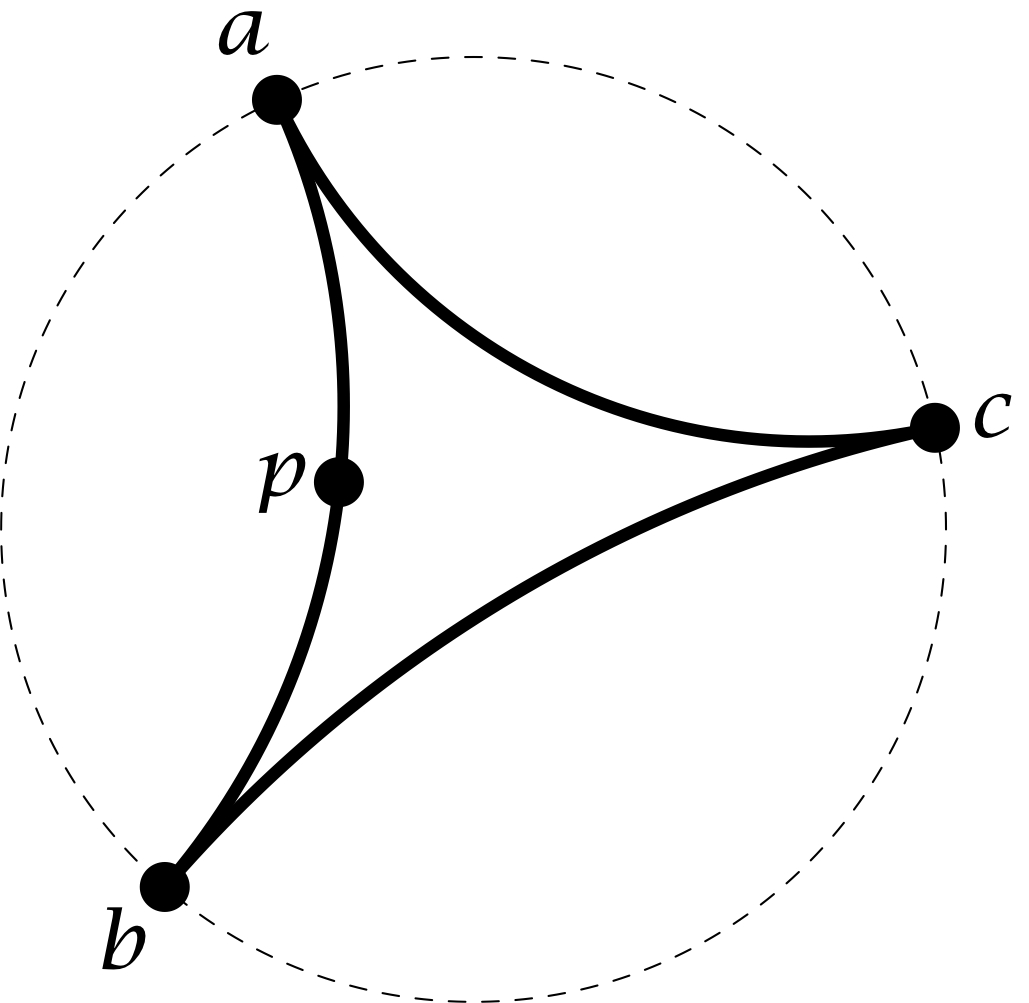
\includegraphics{PDF/idealtriangle.jpg}}\vss}%
\hangindent=-1.85in \hangafter=0 
Any three distinct points $a$, $b$, and~$c$ on $\bdry\hyperbolic^2$ are the vertices of an ideal triangle (with geodesic sides).
%texpreamble
%("  \usepackage{amsmath}
% \usepackage[LY1]{fontenc}
% \usepackage[expert,LY1,mylucidascale]{mylucidabr}
% ");
%defaultpen(  fontcommand("\normalfont") + fontsize(10) ); 
%
%from graph access *;
%unitsize(2cm);
%
%real linethick = 1.5;
%real dotthick = 12;
%dotfactor=12;
%
%real atheta = 2;
%pair a = ( cos(atheta), sin(atheta) );
%
%real btheta = 4;
%pair b = ( cos(btheta), sin(btheta) );
%
%real ctheta = 6.5;
%pair c = ( cos(ctheta), sin(ctheta) );
%
%pair p = (-0.285, 0.1);
%dot( p ); label( "$p$", p, W );
%
%draw( circle((0,0), 1), linewidth(0.25)+dashed );
%
%dot( a ); label( "$a$", a, 2*a );
%dot( b );label( "$b$", b, b );
%dot( c );label( "$c$", c, 1.5*c );
%
%draw( a{-a}..{b}b , linewidth(linethick) );
%draw( b{-b}..{c}c , linewidth(linethick));
%draw( c{-c}..{a}a , linewidth(linethick));
%
Choose a point~$p$ on $\overline{ab}$.
Since the geodesic ray $\overrightarrow{pa}$ is asymptotic to $\overrightarrow{ca}$, there is some $\delta > 0$, such that every point of $\overrightarrow{pa}$ is in the $\delta$-neighborhood of $\overrightarrow{ca}$. Similarly, every point of $\overrightarrow{pb}$ is in the $\delta$-neighborhood of $\overrightarrow{cb}$ (after we enlarge~$\delta$). Therefore, all of $\overline{ab}$ is in the $\delta$-neighborhood of the union of the other two sides. By applying the same argument to the sides $\overline{bc}$ and $\overline{ac}$, we see there is some $\delta$, such that the triangle $abc$ is $\delta$-thin.
}

Since the isometry group $\SL(2,\real)$ acts transitively on the (unordered) triples of distinct points on the boundary, we conclude that every ideal triangle is $\delta$-thin for this same value of~$\delta$. Having vertices on the boundary is the worst-case scenario, so this implies that all geodesic triangles in $\hyperbolic^2$ are $\delta$-thin.
\end{proof}

The following important ``shadowing property'' tells us that ``quasi-geodesics'' are always close to geodesics. Unfortunately, its proof is somewhat lengthy, so we omit it. (See \cref{HyperbolicGeodUnique,HyperbolicLargerC} for some weaker results that are easier.) 
% Maybe should also prove logarithmic distance, since that's not hard? @@@

\begin{thm} \label{CoarseShadowing}
Suppose 
	\begin{itemize}
	\item $X$ is a $C$-coarsely geodesic $\delta$-hyperbolic metric space,
	and
	\item $\{x_0,x_1,\ldots,x_n\}$ is finite sequence of points in~$X$, such that, for all $i,j$ we have:
		$$ \frac{|i - j|}{C} - C \le d(x_i, x_j) \le C|i - j| + C .$$
	\end{itemize}
Then there exists $C' > 0$ \textup(depending only on~$C$ and~$\delta$\textup), such that the set $\{x_0,x_1,\ldots,x_n\}$ is contained in the $C'$-neighborhood of every $C$-coarse geodesic from~$x_0$ to~$x_1$.
\end{thm}

This implies that being Gromov hyperbolic is invariant under quasi-isometry:

\begin{cor}[\csee{HyperbolicQIInvtEx}] \label{HyperbolicQIInvt}
Assume
\noprelistbreak
	\begin{itemize}
	\item $X_1$ and~$X_2$ are coarsely geodesic metric spaces,
	and
	\item $X_1 \QI X_2$.
	\end{itemize}
If $X_1$ is Gromov hyperbolic, then $X_2$ is Gromov hyperbolic.
\end{cor}

\begin{cor}
The fundamental group of any compact manifold~$M$ of strictly negative sectional curvature is Gromov hyperbolic.
\end{cor}

\begin{proof}
Since $M$ is compact, the fundamental group $\pi_1(M)$ acts cocompactly on the universal cover~$\cover M$ of~$M$, so $\pi_1(M) \QI \cover M$ \csee{CocpctActIsQI}. Now apply \cref{NegCurvGromovHyp,HyperbolicQIInvt}.
\end{proof}

This observation allows us to determine precisely which lattices are Gromov hyperbolic:

\begin{prop} \label{WhichLattsHyper}
 $\Gamma$ is Gromov hyperbolic if and only if\/
$\Rrank G = 1$ and either $G/\Gamma$ is
compact, or the unique noncompact simple factor of~$G$ is
isogenous to\/ $\SL(2,\real)$.
 \end{prop}

\begin{proof}[Sketch of proof]
With a bit more theory than has been presented here, it is not difficult to show that Gromov hyperbolic groups never contain a subgroup isomorphic to $\integer \times
\integer$, so we may assume $\Gamma$ is irreducible.

\setcounter{case}{0}

\begin{case}
Assume $G/\Gamma$ is compact.
 \end{case}
 From \cref{CocpctActIsQI}, we know that $\Gamma$ is quasi-isometric to the symmetric space $G/K$ associated to~$G$.
 	\begin{itemize}
	\item If $\Rrank G = 1$, then $G/K$ has negative sectional curvature, bounded away from~$0$, so it is Gromov hyperbolic. 
	\item If $\Rrank G \ge 2$, then $G/K$ contains $2$-dimensional
flats, so it is not Gromov hyperbolic.
	\end{itemize}

\begin{case}
Assume $G/\Gamma$ is not compact.
 \end{case}
 $(\Rightarrow)$ We may assume that $G$ has no compact factors. Let $U$ be a maximal unipotent subgroup of~$\Gamma$. We know that $U$ does not
contain a subgroup isomorphic to $\integer \times
\integer$. Also, since $G/\Gamma$ is not compact, we know $U$ is infinite \csee{GodementConverse}. Therefore, since $U$ is nilpotent (and torsion-free), it is easy to see that $U$ must be cyclic. It can be shown that this implies $G$ is isogenous to
$\SL(2,\real)$.

$(\Leftarrow)$ $\Gamma$ is virtually free, so it is Gromov hyperbolic \csee{FreeGrpsAreHyper}.
 \end{proof}


\begin{exercises}

\item \label{HyperbolicGeodUnique}
Show that the coarse geodesic between two points in a Gromov hyperbolic space is coarsely unique. More precisely, given $C$, show there is some $C' > 0$, such that if $\gamma$ and~$\gamma'$ are two $C$-coarse geodesics with the same endpoints, then $\gamma$ is contained in the $C'$-neighborhood of~$\gamma'$.
\hint{If $a$ and~$b$ are the two endpoints, consider the (degenerate) triangle $abb$.}

\item \label{HyperbolicLargerC}
Show that if $X$ is a $C$-coarsely geodesic $\delta$-hyperbolic space, and $C' \ge C$, then there exists~$\delta'$, such that every $C'$-coarse geodesic from~$a$ to~$b$ is in the $\delta'$-neighborhood of every $C$-coarse geodesic from~$a$ to~$b$.
(This is a generalization of \cref{HyperbolicGeodUnique}.)
\hint{For any point~$c$ on a $C'$-coarse geodesic from~$a$ to~$b$, there is a $C$-coarse triangle $abc$. If $c$ is not in the $\delta$-neighborhood of $\overline{ab}$, then there exist $a',b' \in \overline{ab}$ that are distance less than~$\delta$ from points $a''$ and~$b''$ on $\overline{ac}$ and $\overline{bc}$, respectively, such that $d(a',b') < C + 1$. Bound $d(a',c)$ by noting that $c$ is on the $C''$-coarse geodesic $\overline{a''c} \cup \overline{cb''}$.}

\item \label{FreeGrpsAreHyper}
Show that free groups are Gromov hyperbolic.
\hint{The word metric corresponding to a set of free generators is $0$-hyperbolic.}

\item \label{HyperbolicQIInvtEx}
Prove \cref{HyperbolicQIInvt}.
\hint{Use \cref{CoarseShadowing} to show that coarse triangles in~$X_2$ can be approximated by coarse triangles in~$X_1$.}

\end{exercises}




\begin{notes}

Almost all of the material in this chapter can be found in any treatment of geometric group theory, such as \cite{GhysDelaHarpe-InfGrpsGeomObjs}, \cite{delaHarpe-TopicsGeomGrpThy}, or (more elementary)~\cite{Bowditch-CourseGGT}. A detailed treatment of this and much more is in \cite{BridsonHaefliger}. 

The Lubotzky-Mozes-Raghunathan Theorem \pref{LMRThm} is proved in \cite{LubotzkyMozesRaghunathan} (or see \cite{LubotzkyMozesRaghunathan-CR} for an exposition of the special case where $\Gamma = \SL(n,\integer)$). 

See \cite{Ghys-GrpHyp} for an introduction to the theory of Gromov hyperbolic groups, or \cite{GhysDelaHarpe-GrpsHyp,Gromov-HypGrps} for much more information.
The notion of $\delta$-hyperbolic group is credited to E.\,Rips, who also proved some of the basic properties (such as that they are finitely presented), but much of the foundational work in the subject was done by M.\,Gromov \cite{Gromov-HypGrps}.

\Cref{WhichLattsHyper} is well known.

\end{notes}


\begin{references}{[9]}

\bibitem{Bowditch-CourseGGT}
B.\,Bowditch:
\emph{A Course on Geometric Group Theory}.
%MSJ Memoirs, 16. 
Mathematical Society of Japan, Tokyo, 2006.
ISBN 4-931469-35-3,
\MR{2243589}

\bibitem{BridsonHaefliger}
M.\,Bridson and A.\,Haefliger:
\emph{Metric Spaces of Non-Positive Curvature}.
Springer, Berlin, 1999.
ISBN 3-540-64324-9,
\MR{1744486}

\bibitem{Ghys-GrpHyp}
\'E.\,Ghys: Les groupes hyperboliques, 
\emph{Ast\'erisque} 189-190 (1990) 203--238.
\MR{1099877},
\url{http://www.numdam.org/item?id=SB_1989-1990__32__203_0}

\bibitem{GhysDelaHarpe-GrpsHyp}
\'E.\,Ghys and P.\,de\,la\,Harpe:
Sur les Groupes Hyperboliques d'apr\`es Mikhael Gromov.
%Papers from the Swiss Seminar on Hyperbolic Groups held in Bern, 1988. 
%Progress in Mathematics, 83. 
Birkh\"auser, Boston, 1990.
ISBN 0-8176-3508-4,
\MR{1086648}

\bibitem{GhysDelaHarpe-InfGrpsGeomObjs}
\'E.\,Ghys and P.\,de\,la\,Harpe:
Infinite groups as geometric objects (after Gromov),
in T.\,Bedford, et al., eds.:
\emph{Ergodic Theory, Symbolic Dynamics, and Hyperbolic Spaces (Trieste, 1989)}, 
Oxford Univ. Press, New York, 1991, 
pp.~299--314.
ISBN 0-19-853390-X,
\MR{1130180}

%\bibitem{Gromov-InfGrpsGeomObjs}
%M.\,Gromov:
%Infinite groups as geometric objects,
%\emph{Proc. Internat. Cong. Math. (Warsaw, 1983)}, , Vol. 1, 2385Ð392, 
%PWN, Warsaw, 1984. 
%\MR{0804694}

\bibitem{Gromov-HypGrps}
M.\,Gromov:
Hyperbolic groups,
in  S.\,M.\,Gersten, ed.:
\emph{Essays in Group Theory}, 
Springer, New York, 1987, pp.~75--263.
ISBN 0-387-96618-8,
\MR{0919829}

\bibitem{delaHarpe-TopicsGeomGrpThy}
P.\,de\,la\,Harpe:
\emph{Topics in Geometric Group Theory}.
Univ. of Chicago Press, Chicago, 2000.
ISBN 0-226-31719-6,
\MR{1786869} 

\bibitem{LubotzkyMozesRaghunathan-CR}
 A.\,Lubotzky, S.\,Mozes, and M.\,S.\,Raghunathan:
 Cyclic subgroups of exponential growth and metrics on
discrete groups,
 \emph{Comptes Rendus Acad. Sci. Paris}, Ser.~A, 317
(1993), no.~8, 735--740. 
\MR{1244421},
\maynewline
\url{http://gallica.bnf.fr/ark:/12148/bpt6k5808224h/f739.image}

\bibitem{LubotzkyMozesRaghunathan}
A.\,Lubotzky, S.\,Mozes, and M.\,S.\,Raghunathan:
The word and Riemannian metrics on lattices of semisimple groups,
\emph{Publ. Math. IHES} 91 (2000) 5--53.
\MR{1828742},
\url{http://www.numdam.org/item?id=PMIHES_2000__91__5_0}


\end{references}

